\documentclass[10pt,foldmark,tumble]{leaflet}
\renewcommand*\foldmarkrule{.3mm}
\renewcommand*\foldmarklength{5mm}

\usepackage{amsmath}
\usepackage{blindtext}
\usepackage[T1]{fontenc}
\usepackage{textcomp}
\usepackage{mathptmx}
\usepackage[utf8]{inputenc}
\usepackage[scaled=0.9]{helvet}
\makeatletter

\def\ptmTeX{T\kern-.1667em\lower.5ex\hbox{E}\kern-.075emX\@}
\DeclareRobustCommand{\ptmLaTeX}{L\kern-.3em
        {\setbox0\hbox{T}%
         %\vb@xt@ % :-)
         \vbox to\ht0{\hbox{%
                            \csname S@\f@size\endcsname
                            \fontsize\sf@size\z@
                            \math@fontsfalse\selectfont
                            A}%
                      \vss}%
        }%
        \kern-.12em
        \ptmTeX}

\makeatother
\let\TeX=\ptmTeX
\let\LaTeX=\ptmLaTeX
\usepackage{shortvrb}
\MakeShortVerb{\|}
\usepackage{url}
\usepackage{graphicx}
\usepackage[dvipsnames,usenames]{color}
\definecolor{LIGHTGRAY}{gray}{.9}
\definecolor{ccred}{RGB}{254,128,0}

%%%%\renewcommand{\descfont}{\normalfont}
\newcommand\Lpack[1]{\textsf{#1}}
\newcommand\Lclass[1]{\textsf{#1}}
\newcommand\Lopt[1]{\texttt{#1}}
\newcommand\Lprog[1]{\textit{#1}}

\newcommand*\defaultmarker{\textsuperscript\textasteriskcentered}


\title{\bf Chaostreff}

\author{\Large \bf Chaos Consulting e.V.}
\date{\bf September 12, 2015 }

%%\CutLine*{1}% Dotted line without scissors
%%\CutLine*{6}%  Dotted line with scissors

\AddToBackground{1}{%  Background of a small page
  \put(70,540){
\includegraphics[scale=0.5]{../../gfx/cc_header.png}}}


\AddToBackground{6}{%  Background of a small page
  \put(0,0){\textcolor{ccred}{\rule{\paperwidth}{\paperheight}}}}

%%\AddToBackground{6}{% Background of a large page
%%  \put(0,150){%
%%      \resizebox{.9\paperwidth}{!}{\rotatebox{50}{%
%%        \textsf{\textbf{\textcolor{ccred}{Chaos-Consulting e.V.}}}}}}}



\AddToBackground*{2}{% Background of a large page
  \put(\LenToUnit{.5\paperwidth},\LenToUnit{.5\paperheight}){%
    \makebox(0,0)[c]{%
      \resizebox{.9\paperwidth}{!}{\rotatebox{35.26}{%
        \textsf{\textbf{\textcolor{LIGHTGRAY}{Chaos-Consulting}}}}}}}}


\begin{document}
\maketitle
\section{Übersicht}
Immer am zweiten Samstag im Monat trifft sich der Iserlohner Chaostreff um 15 Uhr in der Karl-Arnold-Str. 28 in 58644 Iserlohn. Das monatliche Treffen ist eine gute Möglichkeit für Interessierte den Chaostreff einmal näher kennen zu lernen. Unsere Mitglieder kommen aus dem gesamten Märkischen Kreis und arbeiten gemeinsam unter anderem an Ihren Projekten, halten Vorträge und entwickeln neue Projektideen.

Am 12. September gibt es Vorträge zu folgenden Themen:
\begin{itemize}
\item Freifunk
\item Chaos-Consulting Verein
\item ...
\end{itemize}

\blindtext

\section{Ablauf}
\blindtext

\section{Lokation}
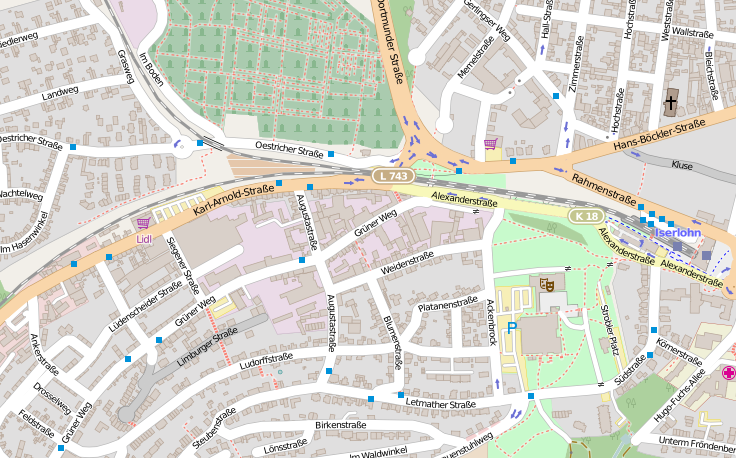
\includegraphics[scale=0.3]{map.png}
\blindtext

\section{Parken}
\blindtext

\blindtext

\blindtext

\blindtext

\blindtext

\blindtext

\blindtext

\hfill
\section{Spenden}
Chaos-Consulting e.V.\\
IBAN: ...\\
BIC: ....\\
\end{document}
